\makeatletter\def\input@path{{../template/vsp-beamer}{../template/minimus}}\makeatother

\documentclass[red,tutorial,sectionpages,shtu]{vsp-beamer}

\graphicspath{{build}{image}{../template/vsp-beamer/assets/}}

\usepackage{minimus-section}
\usepackage{minimus-text}
\usepackage{minimus-math}
\usepackage{minimus-float}
\usepackage{minimus-code}
\usepackage{minimus-colorbox}
\usepackage{minimus-reference}

\title{CS100 Recitation 2}
\subtitle{Git Basics}
\VSPsetspeaker{Yuxuan Li (liyx22025@shanghaitech.edu.cn)}{VSPLab@SIST}
\VSPsetupfootline{CS100 Recitation 2}{Fall 2026}{Yuxuan Li}

%\setkeys{Gin}{draft}

\begin{document}

\VSPtitleframe

\begin{frame}{目录}
    \tableofcontents[hideallsubsections]
\end{frame}

\section{Git是什么}

\begin{frame}{Git是什么}
    Git是一个版本控制软件，它以增量方式记录代码修改，保存完整版本历史！
\end{frame}

\begin{frame}{Git与GitHub}
    \alert{Git并不等同于GitHub}！你完全可以用Git对本地项目进行版本控制，并不需要注册任何账号。
    
    \begin{itemize}
        \item Git是一个运行在本地的版本控制软件。
        \item GitHub则是一个很流行的Git仓库托管平台。
    \end{itemize}

    Git很适合用于多人协作的代码开发，它可以很好地解决版本同步和合并。不过，这需要一个所有人可访问的远程仓库，而GitHub的作用就是提供一个开放的平台用于创建和托管远程仓库。
    
    \alert{许多著名的开源项目都会将它们的仓库托管在GitHub上}！
\end{frame}

\begin{frame}{为什么需要版本控制？}
    哈哈，看起来很眼熟？\alert{请使用Git来管理你的代码吧}！
    \begin{itemize}
        \item 我尝试修改了一些代码，一切都崩溃了，但刚刚明明都还是好的！
        \item 我想做几个实验性的修改，但很害怕把项目搞乱而不敢尝试！
        \item 我想查看上个月的一个问题是如何修复的，但我完全忘记当时改了什么！
        \item 我和我的合作者用微信来传递彼此的代码，两个人还碰巧改了同一个文件！
        \item 我将我的合作者的代码缝合至项目后，无法运行了，搞不清到底是谁的问题！
    \end{itemize}
    版本控制是体面地进行代码开发不可或缺的工具，即便是本地的个人项目也是如此！
\end{frame}

\section{Git：在本地仓库使用}

\begin{frame}{Git安装}
    Git可以通过\code{apt}安装
    \begin{Code}*
        \lstinputlisting{code/install-git.sh}
    \end{Code}
    Git有时需要一个文本编辑器，因此安装一下Vim
    \begin{Code}*
        \lstinputlisting{code/install-vim.sh}
    \end{Code}
\end{frame}

\begin{frame}{Git配置}
    Git在第一次创建提交前需要设置用户名和邮箱
    \begin{Code}*
        \lstinputlisting[firstline=1,lastline=2]{code/git-config.sh}
    \end{Code}
    Git默认搭配的文本编辑器是Nano，可以更换为Vim
    \begin{Code}*
        \lstinputlisting[firstline=3,lastline=4]{code/git-config.sh}
    \end{Code}
\end{frame}

\begin{frame}{Git创建仓库}
    Git仓库（Repository）是Git用来管理一个项目的版本历史的核心结构。
    
    若希望对某个项目使用Git版本控制，就要在该项目的目录下初始化Git仓库，命令是
    \begin{Code}*
        \lstinputlisting[firstline=1,lastline=1]{code/git-init.sh}
    \end{Code}
    完成后，当前目录就会出现一个\code{.git}隐藏目录，所有和版本控制相关的数据都会被存储在该目录中。因此，如果想要移除某个项目的版本控制，只需要简单地删除\code{.git}目录即可。
\end{frame}

\begin{frame}{Git提交更改}
    Git仓库由以下三个重要部分组成
    \begin{itemize}
        \item \alert{工作区}（Workspace）
        \item \alert{暂存区}（Index）
        \item \alert{版本库}（Repository）
    \end{itemize}
    工作区就是你能看到的工作目录。当希望创建一个提交（Commit）时\footnote{Git的版本被称为“提交”，这不涉及到任何远程。}，需要两个步骤：首先需要将工作区的改动添加到暂存区（\alert{工作区}$\to$\alert{暂存区}），暂存区提供了一个中间缓冲区，用于存放准备提交的更改。随后需要将暂存区的改动提交到版本库（\alert{暂存区}$\to$\alert{版本库}），形成一个提交。
\end{frame}

\begin{frame}{Git提交更改}
    \alert{将改动添加到暂存区}（Add），其中\code{.}代表添加当前目录下的所有更改
    \begin{Code}*
        \lstinputlisting{code/git-add.sh}
    \end{Code}
    \alert{将改动提交到版本库}（Commit），其中选项\code{-m}用于写入提交的备注
    \begin{Code}*
        \lstinputlisting{code/git-commit.sh}
    \end{Code}
\end{frame}

\begin{frame}{Git提交更改}
    \alert{Git为何要引入一个中间的暂存区的概念}？这是因为，Git期望每一个提交是最小化的，但实践中，代码修改经常是一个连贯的过程，可能同时修改了多处代码。这时，暂存区的意义就体现出来了，使多个修改可以分步提交：先将一处修改暂存后提交，再将另一处修改暂存后提交。
    
    然而，通过命令行完成很精细地暂存是比较麻烦的，推荐在VSCode中以图形化方式（侧边栏的Source Control）交互完成，你可以精细地选择，甚至可以只暂存同一文件中的一处修改！
\end{frame}

\begin{frame}{Git提交更改}
    \alert{Git只应当追踪源文件的变化}，任何编译输出都应该被忽略
    \begin{itemize}
        \item 编译结果可以自动化产生（如果不能，请让它能），删除后随时可以复现。
        \item 编译的输出文件的体积往往远远大于源代码，且每次编译后都可能会发生变化。
        \item 编译的输出文件通常是二进制，而Git的增量记录不适用于二进制文件！
    \end{itemize}
    这需要在项目的根目录创建一个名为\code{.gitignore}的文件，并写入忽略的内容
    \begin{Code}*
        \lstinputlisting{code/example.gitignore}
    \end{Code}
\end{frame}

\begin{frame}{创建提交}
    \begin{Figure}*
        \includegraphics[scale=0.9]{GitCommit.fig.pdf}
    \end{Figure}
\end{frame}

\begin{frame}{Git添加标签}
    Git允许对一些重要的版本添加标签，以便后续更容易地找到这个版本
    \begin{Code}*
        \lstinputlisting[firstline=1,lastline=1]{code/git-tag.sh}
    \end{Code}
    选项\code{-d}用于删除标签
    \begin{Code}*
        \lstinputlisting[firstline=2,lastline=2]{code/git-tag.sh}
    \end{Code}
\end{frame}

\begin{frame}{添加标签}
    \begin{Figure}*
        \includegraphics[scale=0.9]{GitTag.fig.pdf}
    \end{Figure}
\end{frame}

\begin{frame}{Git查看状态}
    查看当前Git仓库的状态和所在分支（若没有更改，会提示“干净的工作区”）
    \begin{Code}*
        \lstinputlisting{code/git-status.sh}
    \end{Code}
    查看当前Git仓库的版本历史，选项\code{--graph}可以提供更漂亮的输出
    \begin{Code}*
        \lstinputlisting{code/git-log.sh}
    \end{Code}
    当然，你也可以在VSCode的图形界面中更直观地看到这些信息。
\end{frame}

\begin{frame}{Git分支管理}
    Git的版本库从数据结构的角度，可以视为一个有向无环图：
    \begin{itemize}
        \item 每个提交都是图的一个节点。
        \item 每个提交都会记住其父提交，即上一个提交。
        \item 提交对应的节点以类似链表的方式组织起整个版本库。
    \end{itemize}
    \alert{Git分支的本质，就是指向提交的一个指针}。分支指向的提交以及该提交向前溯及的每一个提交，就反映了这个分支的历史。创建多个Git分支，就可以使仓库获得多个不同的发展方向。

    Git默认会创建一个称为\code{master}的分支\footnote{由于一些原因，部分平台改用\code{main}取代\code{master}作为主分支名。}，作为主分支。
\end{frame}

\begin{frame}{Git分支管理}
    创建一个分支
    \begin{Code}*
        \lstinputlisting[firstline=1,lastline=1]{code/git-branch.sh}
    \end{Code}
    切换至一个分支
    \begin{Code}*
        \lstinputlisting[firstline=1,lastline=1]{code/git-checkout.sh}
    \end{Code}
    Git切换分支的本质，就是在切换头指针\code{HEAD}所指向的分支指针！
    
    通常来说，头指针并不直接指向提交：\alert{头指针一般先指向分支指针，这代表当前所处的分支}。
\end{frame}

\begin{frame}{创建分支}
    \begin{Figure}*
        \includegraphics[scale=0.9]{GitBranch.fig.pdf}
    \end{Figure}
\end{frame}

\begin{frame}{切换分支}
    \begin{Figure}*
        \includegraphics[scale=0.9]{GitCheckout.fig.pdf}
    \end{Figure}
\end{frame}

\begin{frame}{Git分支管理}
    查看所有分支
    \begin{Code}*
        \lstinputlisting[firstline=4,lastline=4]{code/git-branch.sh}
    \end{Code}
    有时需要删除分支，可以使用\code{branch}的\code{-d}选项
    \begin{Code}*
        \lstinputlisting[firstline=2,lastline=2]{code/git-branch.sh}
    \end{Code}
    有时需要重命名分支，可以使用\code{branch}的\code{-m}选项
    \begin{Code}*
        \lstinputlisting[firstline=3,lastline=3]{code/git-branch.sh}
    \end{Code}
\end{frame}

\begin{frame}{Git分支管理}
    有时需要创建一个新分支并立即切换，可以使用\code{checkout}的\code{-b}选项
    \begin{Code}*
        \lstinputlisting[firstline=2,lastline=2]{code/git-checkout.sh}
    \end{Code}
    实际上，直接切换到一个提交而非分支也是被允许的，这种头指针绕过分支指针直接指向提交的特殊状态被称为“\alert{分离的头指针}”，该技巧常用于查看一个特定的历史版本，例如
    \begin{Code}*
        \lstinputlisting[firstline=3,lastline=3]{code/git-checkout.sh}
    \end{Code}
    但请注意，切勿在“分离的头指针”的状态下创建提交！
\end{frame}

\begin{frame}{查看历史版本}
    \begin{Figure}*
        \includegraphics[scale=0.9]{GitDetach.fig.pdf}
    \end{Figure}
\end{frame}

\begin{frame}{Git分支合并}
    Git允许在若干不同分支上进行不同的开发，\alert{需要时再将各分支的工作合并}。
    
    Git在合并中能自动处理大部分情况，确有冲突时，会让用户来决定如何解决冲突。

    在\code{master}分支上合并\code{dev}分支
    \begin{Code}*
        \lstinputlisting[firstline=1,lastline=1]{code/git-merge.sh}
    \end{Code}
\end{frame}

\begin{frame}{Git分支合并}
    运行\code{git merge}后，通常可能会出现两种情况
    \begin{itemize}
        \item \alert{快进}（Fast Forward）
        \item \alert{合并}（Merge）：自动合并 / 手动合并
    \end{itemize}
    快进是一种特殊的情形，这适用于\code{master}分支位于\code{dev}分支向前溯及的某个历史提交上。
    
    在这种情况下，只需要将\code{master}分支指针移动到\code{dev}分支指针的位置，就可以完成合并。
\end{frame}

\begin{frame}{分支快进}
    \begin{Figure}*
        \includegraphics[scale=0.9]{GitFastForward.fig.pdf}
    \end{Figure}
\end{frame}

\begin{frame}{Git分支合并}
    自动合并意味着\code{master}和\code{dev}各有新提交，但这些提交的改动并不冲突，例如修改两个文件或修改同一个文件的不同位置，因此Git可以自动处理合并。这种情况下Git会立即创建一个新提交作为合并结果，这个提交非常特殊，它有两个父提交，可以溯及两段不同的历史。
    
    自动合并的过程中会弹出一个Vim界面，这相当于让你输入\code{git commit -m}的提交说明，但是以文件的形式输入。保存文件就可以写入提交说明，默认说明是\code{Merge branch 'dev'}。
\end{frame}

\begin{frame}{分支合并}
    \begin{Figure}*
        \includegraphics[scale=0.9]{GitMerge.fig.pdf}
    \end{Figure}
\end{frame}

\begin{frame}{Git分支合并}
    手动合并意味着\code{master}和\code{dev}各自的新提交存在Git无法自动处理的冲突，例如修改同一个文件的同一位置。这种情况下，合并仍然会进行，命令行会提示需要手动解决冲突，同时文件中会以一种特殊标记标注所有的冲突点。若使用VSCode查看，这类标记会获得特殊高亮。
    \begin{Code}*
        \lstinputlisting{code/merge-conflict.txt}
    \end{Code}
    在逐一解决完所有冲突后，需要手动执行\code{git add}和\code{git commit}创建提交，结束合并窗口。
\end{frame}

\begin{frame}{Git版本回退}
    回退至一个特定版本
    \begin{Code}*
        \lstinputlisting[firstline=1,lastline=1]{code/git-reset.sh}
    \end{Code}
    请注意，在Git中回退版本可能是危险的！你无法回退到一个早期版本然后再重新回到最新版本。因为一个提交能被访问的前提是这条提交链的顶端需要有一个分支指针，若一个提交链的顶端没有分支指针，这个提交链上的所有提交就都消失了（仍存在，但不能用常规方式访问）！
    
    因此，若目的是查看历史版本，请使用\code{git checkout}替代\code{git reset --hard}。
    
    若确实需要回退且不希望丢失提交，\alert{请在回退前创建一个额外的分支挂在提交链顶端}。
\end{frame}

\begin{frame}{回退历史版本}
    \begin{Figure}*
        \includegraphics[scale=0.9]{GitReset.fig.pdf}
    \end{Figure} 
\end{frame}

\begin{frame}{Git版本回退}
    回退可以用选项指定行为，但通常\code{--hard}可以提供预期中最干净的回退
    \begin{Table}[Git回退的选项]!!
        \begin{tblr}{colspec={X[1]X[4]}}
            选项&效果\\
            \code{--soft}&将版本库回退至指定提交。\\
            \code{--mixed}&将版本库回退，并使暂存区与其保持一致（这是默认选项）。\\
            \code{--hard}&将版本库回退，并使暂存区和工作区与其保持一致。\\
        \end{tblr}
    \end{Table}
\end{frame}

\begin{frame}{Git版本回退}
    如果希望撤回刚刚的\code{git commit}（例如提交说明写错了）
    \begin{Code}*
        \lstinputlisting[firstline=2,lastline=2]{code/git-reset.sh}
    \end{Code}
    如果希望撤回刚刚的\code{git commit}和\code{git add}（例如跟踪了不该跟踪的文件）
    \begin{Code}*
        \lstinputlisting[firstline=3,lastline=3]{code/git-reset.sh}
    \end{Code}
    其中\code{HEAD^}代表头指针\code{HEAD}的上一提交。
\end{frame}

\section{Git：和远程仓库交互}

\begin{frame}{GitHub注册与配置}
    GitHub是目前最流行的Git仓库托管平台\footnote{\url{https://www.github.com}}，可以通过GitHub创建远程仓库。

    GitHub注册现在强制要求启用2FA认证，可以选择Microsoft Authenticator，具体来说，你需要在手机上安装这个应用，它会动态生成密钥，你在某些情况下需要输入这组密钥。推荐立即在Settings $\to$ General中将默认的主分支名由\code{main}改为\code{master}，避免不一致带来的麻烦。
\end{frame}

\begin{frame}{GitHub注册与配置}
    GitHub允许通过HTTPS和SSH两种方式与远程仓库交互，\alert{但你只应当使用SSH方式}，连接较为稳定，且免于在每次访问远程时输入密码。为此，你需要先在本地创建一对SSH密钥。

    SSH密钥采用RSA或ECC的加密算法\footnote{RSA基于大质数分解，ECC基于椭圆曲线。}，是一种非对称密钥。
    \begin{itemize}
        \item 密钥是成对的，一把是公钥，一把是私钥。
        \item 你应当将公钥提供给别人，而小心地保管私钥。
        \item 用于签名：使用你的私钥加密的数据，都只能用你的公钥解密。
        \item 用于加密：使用你的公钥加密的数据，都只能用你的私钥解密。
    \end{itemize}
\end{frame}

\begin{frame}{GitHub注册与配置}
    用以下命令生成SSH密钥。选项\code{-t rsa}代表使用RSA，选项\code{-b 4096}代表使用4096位的密钥，\code{-C "my-laptop"}代表密钥的注释，交互中，对每个问题直接按回车保持默认即可。
    
    这会生成公钥\code{\~/.ssh/id_rsa.pub}和私钥\code{\~/.ssh/id_rsa}两个文件。
    \begin{Code}*
        \lstinputlisting[firstline=1,lastline=1]{code/ssh-keygen.sh}
    \end{Code}
    查看公钥文件
    \begin{Code}*
        \lstinputlisting[firstline=2,lastline=2]{code/ssh-keygen.sh}
    \end{Code}
    复制显示的内容，在GitHub的Settings $\to$ SSH and GPG keys中点击New SSH Key，将复制的内容粘贴到Key中，将Title留空（Title会自动从密钥注释中被识别），随后点击确定就可以了。
\end{frame}

\begin{frame}{Git克隆远程仓库}
    你可以将远程仓库克隆到本地
    \begin{Code}*
        \lstinputlisting{code/git-clone.sh}
    \end{Code}
    部分Git仓库内会存在Git子模块，你需要在\code{git clone}时添加\code{--recursive}选项。
    
    如果在克隆时忘记加上这个选项，可以在克隆后执行以下命令拉取子模块。
    \begin{Code}*
        \lstinputlisting{code/git-submodule.sh}
    \end{Code}
\end{frame}

\begin{frame}{Git添加远程仓库}
    你需要首先在GitHub上手动创建一个远程仓库，为了后续使用的便利，\alert{不要让它自动生成任何文件}，包括\code{README}和\code{LICENSE}（这些可以在本地添加），确保这是一个干干净净的空仓库。

    添加一个远程仓库
    \begin{Code}*
        \lstinputlisting[firstline=1,lastline=1]{code/git-remote.sh}
    \end{Code}
    查看所有远程仓库
    \begin{Code}*
        \lstinputlisting[firstline=2,lastline=2]{code/git-remote.sh}
    \end{Code}
    远程仓库的名称可以是任意的，但\code{origin}是默认的远程仓库名称。
\end{frame}

\begin{frame}{Git添加远程仓库}
    删除一个远程仓库
    \begin{Code}*
        \lstinputlisting[firstline=3,lastline=3]{code/git-remote.sh}
    \end{Code}
    修改一个远程仓库的名称
    \begin{Code}*
        \lstinputlisting[firstline=4,lastline=4]{code/git-remote.sh}
    \end{Code}
    修改一个远程仓库的目标
    \begin{Code}*
        \lstinputlisting[firstline=5,lastline=5]{code/git-remote.sh}
    \end{Code}
\end{frame}

\begin{frame}{Git使用远程仓库}
    Git和远程仓库的交互主要有下面三条命令
    \begin{itemize}
        \item \code{git push}，将本地分支的提交，\alert{推送}到远程分支，用于上传（Push）。
        \item \code{git pull}，将远程分支的提交，\alert{拉取}到本地分支，用于下载（Pull）。
        \item \code{git fetch}，\alert{获取}远程分支的状态，用于刷新下载源（Fetch）。
    \end{itemize}
    总结：上传用\code{git push}命令，下载用\code{git pull}命令，刷新用\code{git fetch}命令！
\end{frame}

\begin{frame}{Git使用远程仓库}
    推送本地分支到远程
    \begin{Code}*
        \lstinputlisting[firstline=1,lastline=1]{code/git-push.sh}
    \end{Code}
    拉取远程分支到本地
    \begin{Code}*
        \lstinputlisting[firstline=1,lastline=1]{code/git-pull.sh}
    \end{Code}
    获取远程分支（但不更新本地分支）
    \begin{Code}*
        \lstinputlisting[firstline=1,lastline=1]{code/git-fetch.sh}
    \end{Code}
\end{frame}

\begin{frame}{Git使用远程仓库}
    当一个分支第一次向远程推送时，需要手动关联本地分支和远程分支
    \begin{Code}*
        \lstinputlisting[firstline=2,lastline=2]{code/git-push.sh}
    \end{Code}
    通过下面的配置，可以自动关联远程分支
    \begin{Code}*
        \lstinputlisting[firstline=3,lastline=3]{code/git-push.sh}
    \end{Code}
\end{frame}

\begin{frame}{Git使用远程仓库}
    实际上，\code{git pull}可以分解为\code{git fetch}和\code{git merge}两个步骤
    \begin{itemize}
        \item 第一步，\code{git fetch}的目的是刷新远程分支的本地副本\code{origin/master}。
        \item 第二步，\code{git merge}的目的是将\code{origin/master}合并到\code{master}。
    \end{itemize}
    如果远程分支和本地分支间发生了偏离，直接使用\code{git pull}命令将无法完成，其默认只允许快进。这时，你就需要通过\code{git fetch}命令和\code{git merge}命令手动拉取并合并远程分支。
    
    在实践中，请尽量避免这种情况！在多人合作中，每个人应当只在自己的分支上工作（例如命名为\code{liyx}和\code{lichf}）。由一个人负责定期合并到\code{master}分支，随后各自再同步\code{master}分支。
\end{frame}

\begin{frame}{关于Gradescope的使用提示}
    \begin{columns}
        \begin{column}{0.48\textwidth}\setlength{\parskip}{6pt}%
            \begin{itemize}
                \item 在GitHub上创建一个\alert{私有}仓库。
                \item 提交方式选择GitHub。
                \item Repository选择该次作业的仓库。
                \item Branch选择用于提交的分支。
            \end{itemize}
        \end{column}
        \begin{column}{0.48\textwidth}
            \begin{Figure}*
                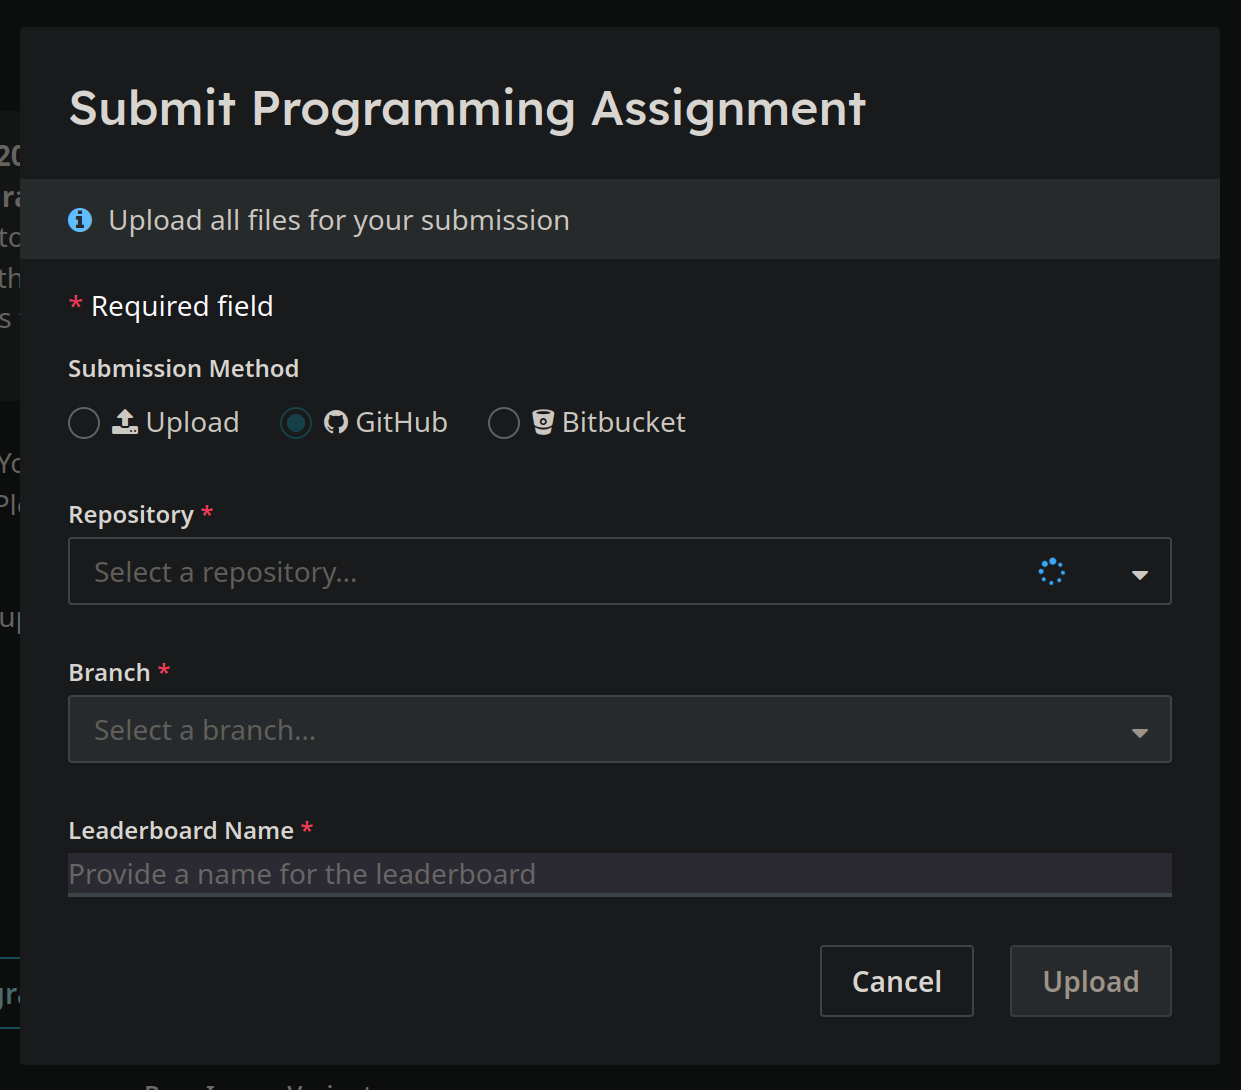
\includegraphics[width=\linewidth]{gradescope.png}
            \end{Figure}
        \end{column}
    \end{columns}
\end{frame}

\section{总结}

\begin{frame}
    \alert{欢迎关注我的GitHub账号}：\url{https://github.com/liyuxuan3003}
\end{frame}


\VSPendframe{}

\end{document}
